% REVISÃO DE LITERATURA--------------------------------------------------------

\chapter{REVISÃO DE LITERATURA}
\label{chap:fundamentacaoTeorica}

Nesta seção, será descrita a revisão de literatura sobre redes neurais, \textit{deep learning} e redes neurais convolucionais.
\par Na \autoref{chap:redeneural} é apresentado os conceitos básicos de redes neurais, mostrando sua composição e funções que influenciam no seu comportamento. Também é defino a estura da rede neural \textit{Perceptron} e os mais comuns tipos de redes neurais.
\par A \autoref{chap:deeplearning} explica o conceito de \textit{deep learning}, a constituição de uma CNN, as operações de convolução, \textit{pooling} e \textit{soft max}, a função de ativação \textit{ReLu}, a técnica de \textit{dropout} e as camadas totalmente conectadas.  

\section{Rede neural}
\label{chap:redeneural}
Rede neural artificial pode ser definida como sendo um conjunto interconectado de elementos básicos de processamento \cite{Gurney1997}. Seu funcionamento é inspirado na capacidade de aprendizado do cérebro animal, que possui uma imensa estrutura com capacidade de definir regras a partir de experiências, que vão ocorrendo durante a vida, gerando ligações físicas (sinapses) mais fortes, aprimorando assim o que foi aprendido \cite{haykin2001}.
\begin{citacao}
  Uma rede neural é um processador maciçamente paralelo e distribuído, constituído de unidades de processamento simples, que tem a propensão natural para armazenar conhecimento experimental e torna-ló disponível para uso. Ela se assemelha ao cérebro em dois aspectos: o conhecimento é adquirido pela rede a partir de seu ambiente por meio de um processo de aprendizagem; forças de conexão entre neurônios, definidos como pesos sinápticos, são utilizados para armazenar o conhecimento adquirido \cite{haykin2001}.
\end{citacao}

\par Dadas essas características, as redes neurais vem sendo amplamente utilizadas para resolução de problemas que não possuem uma resolução trivial, como a classificação de imagens \cite{imaginetArticle}, a identificação de câncer de pele \cite{esteva2017dermatologist}, tomada de decisão no mercado de ações \cite{gambogi2013aplicaccao}, e entre outras áreas. Essa versatilidade de áreas em que é utilizada ocorre devido a sua generalidade na maneira de encontrar pontos no problema que devem ter mais destaque, características mais relevantes que são identificada pela rede durante seu processo de aprendizagem, sendo reavaliadas pela própria rede em cada instância testada. Como dito por \citeonline{zhang2000neural}, as redes neurais possuem a habilidade de se adaptar aos dados para realizar as classificações sem a necessidade de apontar explicitamente o que deve ser observado no modelo.
\par Segundo \citeonline{Kriesel2007NeuralNetworks} uma rede neural pode ser descrita por três elementos:
\begin{itemize}
\item Unidades simples de processamento, ou neurônios.
\item Elos de conexão entre os neurônios (sinapses).
\item A importância entre a conexão de um neurônio com outro, descrita por uma função de peso \textit{w}.
\end{itemize}
\par Uma rede neural pode ser descrita matematicamente pela tríplice ($N$,$V$,$w$), onde $N$ é um conjunto de neurônios, $V$ é um conjunto de conexões entre os neurônios definida por $V = \{($i,$j) \,|\, $i,$j \in N \}$ e $w$ é a função que determina o peso das conexões definida por $w: V \implies \mathbb{R}$, descrita em $w(i,j)$.
\subsection{Neurônio}
\citeonline{haykin2001} define o neurônio como a unidade de processamento de informação que é primordial para o funcionamento de uma rede neural artificial. É nele que ocorre o processamento das entradas, e o redirecionamento da saída, indicando onde irá influenciar tal processamento.
\par Na \autoref{fig:neuronio} é possível identificar os três elementos fundamentais de um neurônio:

\begin{figure}[H]
  \centering
  \caption{Modelo de um neurônio, contendo as entradas, funções de peso, função somadora, o \textit{bias}, função de ativação da saída.}
  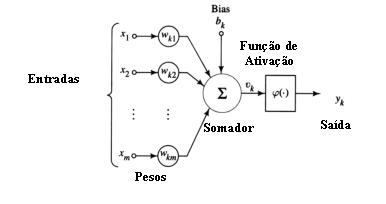
\includegraphics[width=300pt]{dados/figuras/neuron}
  \fonte{imagem retirada do \textit{Google}\protect\footnotemark}
  \label{fig:neuronio}
\end{figure}

\footnotetext{http://www.gsigma.ufsc.br/popov/aulas/rna/neuronio\_artificial/neuronio\_artificial.jpg, acessada em 02 de junho de 2017, ás 18:53}
\begin{itemize}
\item O fluxo de entrada dos dados, sendo ele um conjunto de conexões que serão sujeitas a função de peso, para ser feito o uso na função somadora \cite{haykin2001}. As conexões podem se originar tanto de uma entrada de dados na rede, quanto de neurônios que estão localizados em camadas superiores.
\item A função somadora é responsável por realizar o processamento do fluxo de entrada.
Um exemplo desse tipo de função é a soma dos pesos \cite{Kriesel2007NeuralNetworks}, a função realiza a multiplicação do peso $w_{kj}$ com a entrada $x_j$, e depois realiza a soma das $m$ entradas do neurônio representada pela função matemática:
\par \[u_k = sum_{j=1}^{m} w_{kj}x_j\]
\par O resultado dessa etapa é propagado pela rede dados os critérios da função de ativação.
\item A função de ativação é responsável por restringir a abrangência do dado gerado pelo processamento do neurônio. Foi identificado por \citeonline{haykin2001} três tipos básicos de função de ativação sendo elas:
  \begin{itemize}
    \item \textbf{Função de limiar}:
\[ f(x)= \begin{cases} 1&se \ x \ge 0 \\ -1 & se\ x < 0 \end{cases} \]
      \par É conhecido na literatura como função de \textit{Heaviside}, definindo a saída de maneira binaria.
    \item \textbf{Função linear por partes}: 
\[ f(x)= \begin{cases} 1&se \ x \ge 1 \\x & se\ 0\le x < 1 \\ 0 & se\ x < 0 \end{cases} \]
      \par Esse tipo de função pode ser analisada como uma tentativa de simulação de um amplificador não linear, tendo sua área variável e seus pontos de saturação. 
    \item \textbf{Função Sigmoide}: 
\[ f(x)= \frac{1}{1 + exp(-av)} \]
      \par Esse tipo de função de ativação é o mais utilizado na construção de redes neurais artificiais \cite{haykin2001}. É definida por uma função crescente não linear, quando seu parâmetro de curva se aproxima do infinito, apresenta comportamento semelhante a funções de limiar.
  \end{itemize}
\end{itemize}
\par O modelo neural da figura acima também inclui um \textit{bias} $(b_k)$ aplicado externamente. Tem como função aumentar ou diminuir a entrada mínima de dados. Defini um limiar no neurônio e pode ser utilizado para o cálculo da função de ativação. 
\par Dado as iteração, a \textit{bias} e os pesos da entrada podem ser modificados pelo processo de aprendizagem, aprimorando sua resposta conforme a rede é treinada.  
\subsection{Processos de aprendizagem}
A habilidade que se destaca de uma rede neural é a aprendizagem, adaptando-se aos dados que estão em seu ambiente, para melhorar o seu desempenho. Essa habilidade vem do processo de aprendizagem da rede neural artificial, que é definido por \citeonline{Demuth:2014:NND:2721661} como o procedimento de ajuste das funções de pesos e dos \textit{bias} dos neurônios da rede, acontecendo na etapa de \textit{"treino"} da rede e tem como objetivo preparar a rede para executar uma tarefa. 
\par Podemos dividir o processo de aprendizagem em três categorias principais sendo elas:
\begin{itemize}
\item \textbf{Aprendizado supervisionado:} método no qual uma parte da base é utilizada para treinar a rede. Assim após cada processamento é verificado o resultado da classificação, e se necessário são feitas correções nos pesos dos neurônios que influenciaram esse resultado, para assim reforçar uma classificação boa ou corrigir uma classificação ruim.
\item \textbf{Aprendizado por reforço:} método similar ao aprendizado supervisionado, tendo como diferença a forma de avaliação. Como dito por \citeonline{kaelbling1996reinforcement}, a principal diferença entre aprendizagem supervisionada e a aprendizagem por reforço, é que o aprendizado por reforço não apresenta conjuntos de saídas corretos e errados, e após cada ação é aplicado uma taxa de correção e indicado os estados seguintes, mas não é informado qual escolha teria sido a melhor para o caso.
\item \textbf{Aprendizado não-supervisionado:} método no qual não existe um avaliador ou dados pré-definido informando a classe da entrada, a própria rede é responsável por agrupar os dados, os ajustes dos pesos e dos \textit{bias} é feito apartir das entradas. A rede basicamente aprende como categorizar a entrada de dados em uma quantidade finita de classes. 
\end{itemize}	
\subsection{\textit{Perceptron}}
O \textit{perceptron} é tido como a forma mais simples de rede neural para classificar duas classes que são linearmente separáveis \cite{haykin2001}. Como essa rede é composta por um único neurônio com pesos de conexões e \textit{bias} ajustáveis está limitado a classificar a entrada apenas em duas classes. 
\par A rede é inicializada com pesos aleatórios, e após a execução de cada entrada sua saída é comparada com o resultado esperado, obtendo assim um sinal de erro, que é utilizado para fazer ajustes nos pesos. Como ocorre nos processos de aprendizado supervisionado.
\par Uma generalização do \textit{perceptron}, é o perceptron de múltiplas camadas (no inglês \textit{multiple layer perceptron}, MLP). Onde o MLP é configurado em no mínimo três camadas, onde a primeira delas é a camada de entrada, em que ocorrem a entrada dos dados na rede, e a última é a camada de saída onde está contida a classificação da entrada. As camadas intermediárias tem a função de analisar características mais complexas da entrada, dando possibilidade de uma melhor classificação.
\par O método de aprendizagem utilizado pelo \textit{perceptron} de múltiplas camadas é conhecido como \textit{error backpropagation} (algorítimo de retropropagação de erro) \cite{haykin2001}. Para isso, utiliza do método de aprendizado supervisionado de correção por erro. Quando é identificada a necessidade de ajuste nos pesos, ocorre uma 
retropropagação nos neurônios que influenciaram a classificação, ajustando seus pesos 
e \textit{bias}.
\subsection{Tipos de redes}
Para problemas mais complexos, redes com apenas um neurônio tendem a não resolve-los. Geralmente é necessário ter vários deles trabalhando em paralelo (uma camada de neurônios) \cite{Demuth:2014:NND:2721661}. \cite{haykin2001} descreve três classes de arquitetura de rede que geralmente são encontradas:
\begin{itemize}
\item \textbf{Redes alimentadas adiante de uma camada:} essa classe é a forma mais simples de rede em camada, na qual se tem uma camada de dados e uma camada de neurônios (camada de processamento), que também é a camada de saída, como na \autoref{fig:umacamada}. A camada de entrada de dados não é contada, pois nela não ocorre processamento.
\begin{figure}[H]
  \centering
  \caption{Exemplo de rede alimentada adiante de uma camada.}
  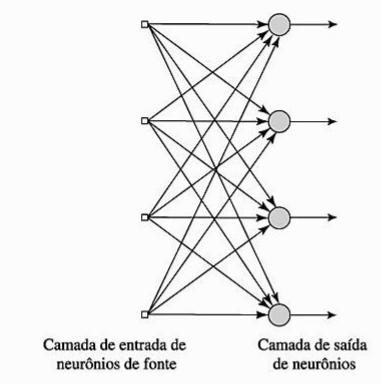
\includegraphics[width=180pt]{dados/figuras/uma_camada}
  \fonte{\cite{haykin2001}}
  \label{fig:umacamada}
\end{figure}

\item \textbf{Redes alimentadas diretamente com múltiplas camadas:} essa classe de rede, é também alimentada adiante, mas possui uma ou mais camadas ocultas. As camadas ocultas estão localizadas entre a camada de entrada de dados e a camada de saída. Ao adicionar camadas ocultas na rede é  possível ter acesso a características mais específicas da entrada, melhorando o resultado da rede.
\par Como representado na \autoref{fig:multicamada}, nesse modelo cada camada só fornece dados à camada posterior, e reciprocamente, só recebe dados da camada anterior. Exemplificando, a camada de entrada recebe os dados e formata a saída para a entrada da camada seguinte, a primeira camada oculta processa os dados fornecidos pela camada de entrada e o formata para a camada seguinte. Esse processo continua até chegar na camada de saída, conhecida também como camada final, a saída produzida por essa camada contém a resposta global produzida pela rede para a entrada fornecida na camada inicial.
\begin{figure}[H]
  \centering
  \caption{Exemplo de rede alimentada diretamente de múltiplas camadas.}
  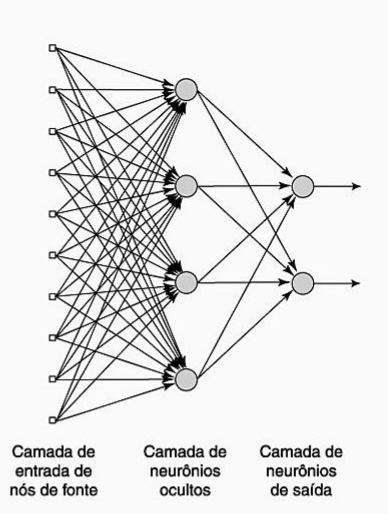
\includegraphics[width=180pt]{dados/figuras/multi_camadas}
  \fonte{\cite{haykin2001}}
  \label{fig:multicamada}
\end{figure}
\item \textbf{Redes recorrentes:} essa classe de arquitetura se diferencia das anteriores pelo fato de possuir pelo menos uma camada com realimentação, ou seja, a saída da camada serve de entrada para a mesma, exemplo \autoref{fig:retroalimentacao}. Os operadores de atraso unitário, representados na imagem pelo símbolo $z^{-1}$, são aplicados nas conexões de realimentação modificando de maneira dinâmica e não linear os valores informados. É dito que a rede possui uma auto-realimentação quando a saída de um neurônio realimenta a sua entrada.
\begin{figure}[H]
  \centering
  \caption{Exemplo de rede retroalimentada.}
  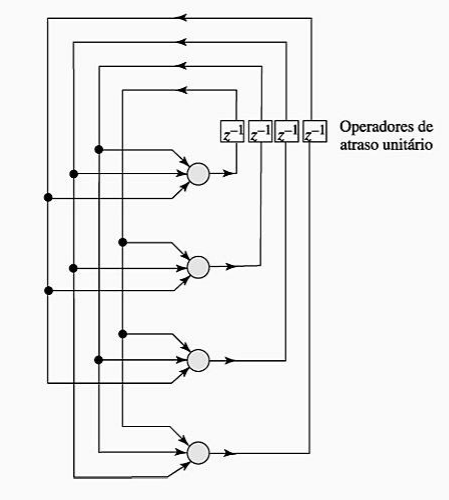
\includegraphics[width=180pt]{dados/figuras/retroalimentacao}
  \fonte{\cite{haykin2001}}
  \label{fig:retroalimentacao}
\end{figure}
\end{itemize}
\section{\textit{Deep learning}}
\label{chap:deeplearning}
\textit{Deep learning} pode ser definido como uma hierarquia de "\textit{conceitos}"\  de aprendizagem, em que "\textit{conceitos}"\  complexos se originam de grupos formados por "\textit{conceitos}"\  mais simples. Se representar esses "\textit{conceitos}"\  em um grafo, é possível ver como um "\textit{conceito}"\  é montado baseado no outro, como se possuíssem muitas camadas \cite{Goodfellow-et-al-2016}.

\begin{citacao}
    \textit{Deep learning} permite que modelos computacionais compostos de múltiplas camadas de processamento aprendam representações de dados com múltiplos níveis de abstração.
    %[...].
    %        Esses métodos tem drasticamente melhorado o estado-da-arte em reconhecimento de fala, reconhecimento visual de objetos, detecção de objetos e muitos outros domínios como na medicina.
   O  \textit{deep learning} descobre estruturas complexas em vastos conjuntos de dados com o uso do algoritmo de retropropagação para indicar como a máquina deve mudar seus parâmetros internos que são utilizados para computar a representação resultante da camada anterior em cada camada \cite{lecun2015deep}.
\end{citacao}

\par \citeonline{bengio2013representation} categoriza o \textit{deep learning} como um método de aprendizagem de representação (do inglês, \textit{representation learning}). Métodos ditos como \textit{representation learning} são capazes receber dados sem tratamento como entrada e a partir de processamentos internos encontrar automaticamente características relevantes para realizar a classificação. Na qual, para o \textit{deep learning}, cada camada oculta de processamento produz uma nova representação, podendo ser descrito como um método de aprendizado de multi representações. Dessa maneira a entrada pode ser uma imagem, descrita em um mapa de \text{bits}, na qual a primeira camada analisa informações mais superficiais, como contornos ou formas em certas áreas das imagens. Já na segunda camada seriam identificados padrões avaliando certas disposições de bordas ou formas em partes da imagem, ignorando pequenas variações. Na terceira camada seria identificado os padrões que se assemelham a partes de objetos conhecidos, e nas camadas posteriores seriam avaliados uma quantidade maior de padrões até chegar ao ponto de realizar a classificação dos objetos contidos na imagem \cite{lecun2015deep}.

\par Por essa versatilidade o \textit{deep learning} vem resolvendo diversos problemas onde as características não estão perceptíveis. Classificação e identificação de objetos \cite{farabet2013learning} e reconhecimento de fala \cite{hinton2012deep} são problemas que vem sendo resolvidos pelo \textit{deep learning}.
\par Na área de classificação de imagem uma técnica de \textit{deep learning} muito utilizado é a rede neural convolucional (do inglês, \textit{convolutional neural network}, CNN). Como mostrado por \citeonline{imaginetArticle}, a CNN vem atualizando o estado da arte na área.

\subsection{Redes neurais convolucionais}
Como descrito por \citeonline{lecun1989backpropagation} redes neurais convolucionais são um tipo especializado de rede neural para processamento de dados que se organizam em grade (ou matriz), tendo como um exemplo de entrada uma imagem, uma matriz de \textit{bits}.
\par Elas possuem o nome de rede convolucional pois, em algumas de suas camadas ocultas ela aplica a operação de convolução. Outra operação muito utilizada nessas redes é a operação de \textit{pooling} \cite{Goodfellow-et-al-2016}.
\par Uma camada de uma rede neural convolucional geralmente é composta de três fases: a primeira fase onde são aplicadas diversas convoluções em paralelo na mesma imagem gerando um conjunto de ativações lineares; a segunda fase propõem a aplicação de uma função de ativação não linear, sendo a unidade linear de correção (do inglês \textit{rectified linear unit}, ReLU) muito utilizada atualmente \cite{lecun2015deep}; no terceiro e último estágio é utilizado uma função de \textit{pooling} para modificar o dado que será fornecido para a próxima camada.    


\subsubsection{Operação de convolução}
Camadas de convolução são baseadas essencialmente na operação de convolução. Segundo \cite{Goodfellow-et-al-2016}, a operação de convolução é descrita por uma operação que ocorre entre duas funções, podendo ser especificada da seguinte maneira:\[s(t) = (x*w)(t)\] %TODO explicar o valor de t


Em redes convolucionais os argumentos da função de convolução são geralmente compostos pela entrada de dado ($x$) e o \textit{kernel} ($w$) utilizado para a modificação. Sua saída é um mapa de características (\textit{feature maps}).

\par Assim, a entrada de dados normalmente é uma matriz, nesse caso uma imagem. O \textit{kernel} utilizado também costuma ser uma matriz de parâmetros que podem ser ajustados pelo processo de aprendizagem (retropropagação). Como saída, cria uma matriz de dados com algumas características ressaltadas.

\par A operação de convolução é uma maneira eficiente de descrever transformações para serem aplicadas em áreas menores mantendo a linearidade, em todo o dado de entrada. Como levantado por \citeonline{Goodfellow-et-al-2016}, para realizar uma operação de subtração entre os \textit{pixels} de uma imagem, para encontrar as bordas como visto na \autoref{fig:convolution}, é necessário uma quantidade muito menor de computação para obter o resultado desejado quando é utilizado a convolução.

\begin{figure}[H]
  \centering
  \caption{Exemplo da aplicação de operações para encontrar as bordas verticais de uma imagem. A esquerda a imagem normal em escala cinza e a direita a imagem aplicada a operação subtração dos \textit{pixeis} vizinhos.}
  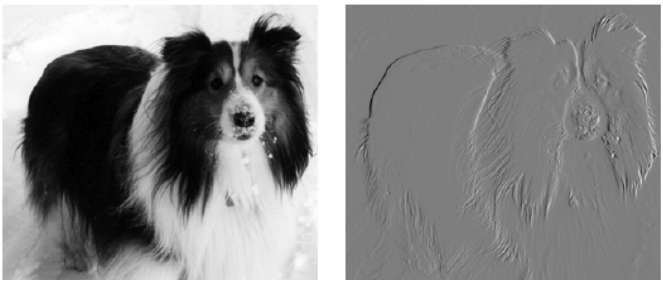
\includegraphics[width=400pt]{dados/figuras/convolution}
  \fonte{\cite{Goodfellow-et-al-2016}}
  \label{fig:convolution}
\end{figure}


\subsubsection{ReLu}

Neurônios com função de ativação ReLu (do inglês, \textit{rectified linear unit}), vem sendo utilizados em redes neurais alimentadas adiante dado seu baixo custo de processamento \cite{glorot2011deep}. Como visto na \autoref{fig:relu}, a ReLu se mantém muito próxima de uma função linear, sendo a única diferença que metade do seu domínio é 0. Isso ocorre nos neurônio que não estão ativos, assim não participando dos processamentos dos dados e das correções que ocorrem na fase de \textit{back propagation}.
\par Sua função é descrita por pela equação $g(z)=max\{0,z\}$, no qual o $z$ no contexto de CNN é a taxa de correção, calculada pelas saídas e as \textit{bias}.
\begin{figure}[H]
  \centering
  \caption{Gráfico da função de ativação não linear ReLu.}
  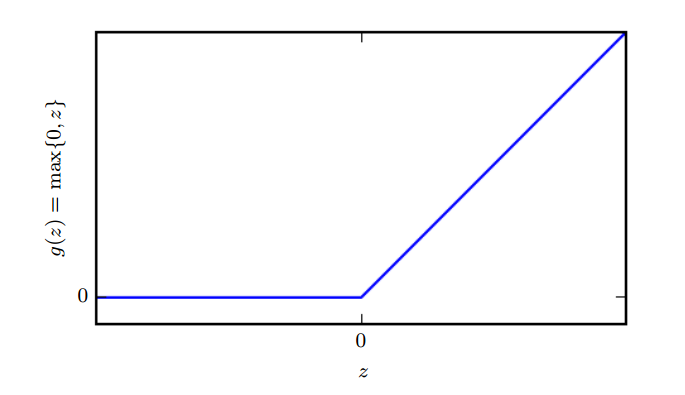
\includegraphics[width=400pt]{dados/figuras/relu}
  \fonte{\cite{Goodfellow-et-al-2016}}
  \label{fig:relu}
\end{figure}

\subsubsection{Operação de \textit{pooling}}
A aplicação da função de \textit{pooling} para modificar o dado de entrada, ajuda a tornar o modelo classificador adaptado a pequenas translações da entrada \cite{Goodfellow-et-al-2016}. Dessa forma a aplicação dessa operação permite identificar se o objeto está contido na imagem independente do local que aparece e das dimensões que apresenta. Essa característica se torna muito eficaz para ser aplicada em redes que necessitam dessa variabilidade de padrões de posição para uma mesma classe.

\par Exemplificando, em uma carta a aplicação da operação de \textit{pooling} permite a rede identificar os números do código postal que estão escrito a mão, mesmo que estes não estejam localizados no mesmo local, ou inclinação de cada respectiva imagem, como exemplo na \autoref{fig:pooling}. 
\begin{figure}[H]
  \centering
  \caption{Exemplo de como é feito a ativação de um neurônio na camada de \textit{pooling}.}
  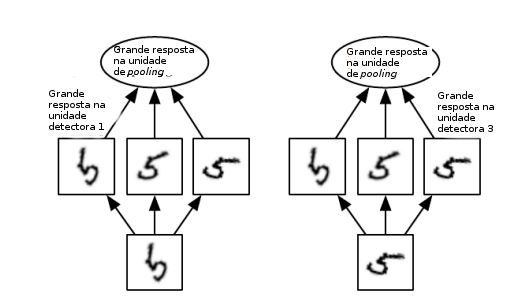
\includegraphics[width=200pt]{dados/figuras/pooling}
  \fonte{\cite{Goodfellow-et-al-2016}}
  \label{fig:pooling}
\end{figure}

% \subsection{Camadas totalmente conectadas}
% As camadas totalmente conectadas são utilizadas nas CNN para realizar a segregação e classificação dos dados aprendidos nas camadas de convolução. Geralmente estão localizadas no fim da rede neural e utilizam da função de ativação ReLu entre suas camadas. Na camada de saída é aplicado a função de \textit{softmax} para ser obtido a classificação da entrada.
% \par O processo de aprendizagem é realizado por meio do \textit{back propagation}, na qual o dado   

\subsubsection{\textit{Dropout}}
Um dos grandes problemas no uso de CNN é o \textit{overfitting}, que ocorre quando a base disponível para o treino é pequena ou quando a rede neural possui muitas camadas. Uma estratégia utilizada por \citeonline{imaginetArticle} é a aplicação da técnica de \textit{dropout} em algumas camadas da rede.
\par \citeonline{srivastava2014dropout} define o termo \textit{dropout} como a remoção temporária de alguns neurônios da rede, junto com suas conexões de entradas e saídas como é possível visualizar na \autoref{fig:dropout}. Essa operação, que remove virtualmente o neurônio da rede neural, ocorre somente na fase de treino, em que quando é ativada no neurônio o exclui do processo de aprendizagem da rede. 
\begin{figure}[H]
  \centering
  \caption{Exemplo da aplicação do \textit{dropout} em uma rede neural. Na imagem (1) apresenta uma rede normal sem remoção de neurônio. Na imagem (2) mostra a rede com o \textit{dropout} ativado em alguns neurônios, os removendo temporariamente.}
  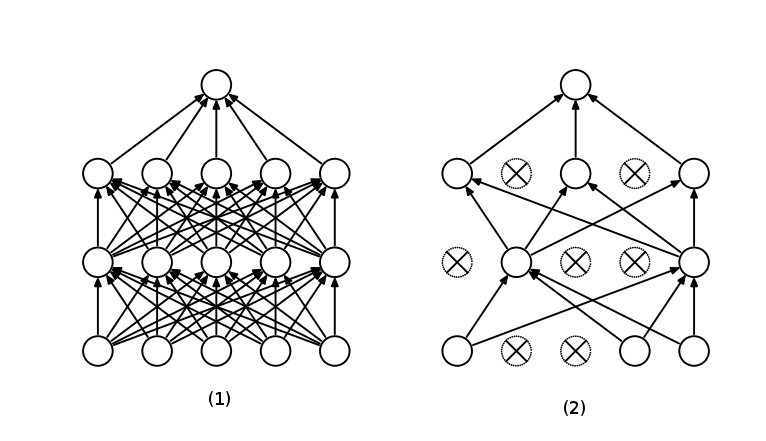
\includegraphics[width=400pt]{dados/figuras/dropout}
  \fonte{\cite{srivastava2014dropout}}
  \label{fig:dropout}
\end{figure} 
\par Essa operação vem com o intuito de reduzir o \textit{overfitting}. A redução do tempo de execução e o aprendizado de atributos mais relevantes pela rede são outras características que se destacam quando aplicada a técnica de \textit{dropout}.

% \subsubsection{\textit{Softmax}}

%TODO esplicar sobre dropout e sofmax e fullconected layers